\section{Data Analysis}

brief explaination of the signature, selection cuts, few words about acceptances, image of signal region and control region.

\begin{figure}[h]
  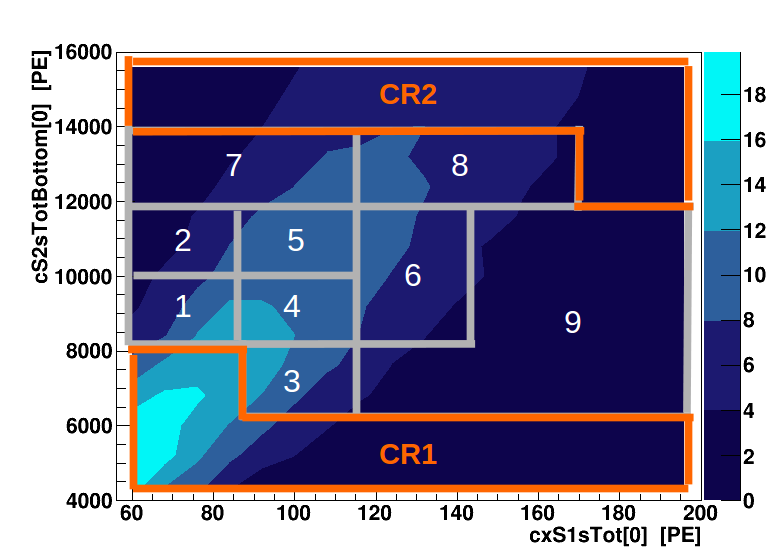
\includegraphics[width=\linewidth]{images/bkg_in_sr.png}
  \caption{Signal region and control region.}
  \label{fig:SR}
\end{figure}

\begin{figure}[h]
  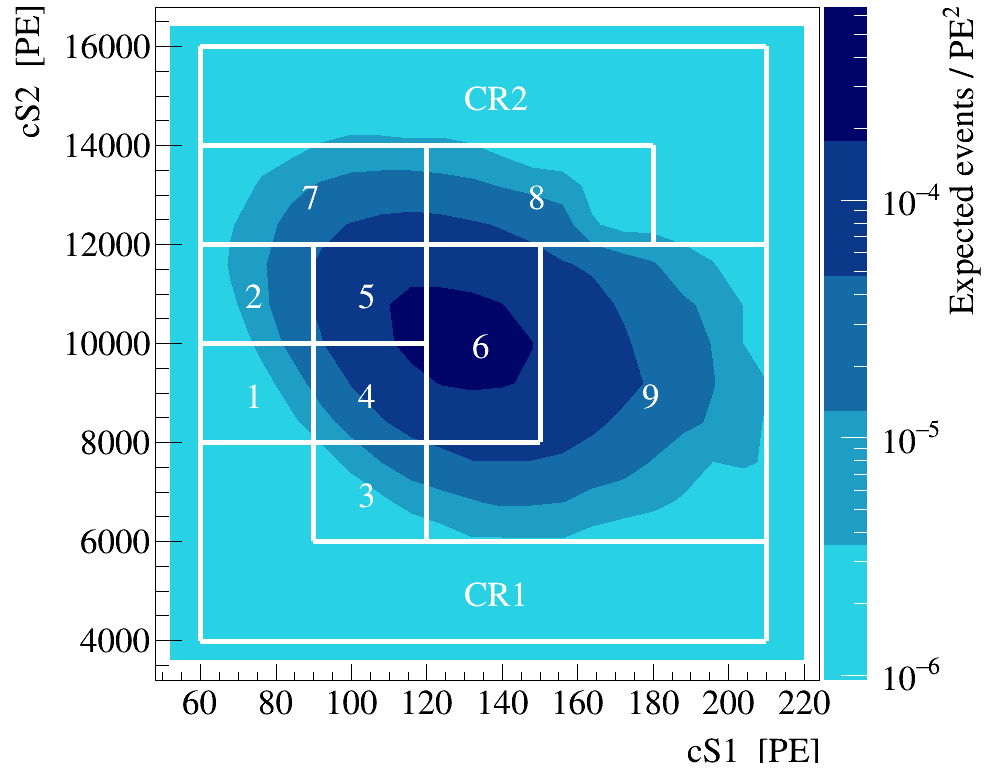
\includegraphics[width=\linewidth]{images/wimp_in_sr.png}
  \caption{Signal region and control region, for WIMP of mass 100~GeV.}
  \label{fig:SR2}
\end{figure}


\subsection{Signal Simulation} 

description of the simulated signal, few words about cross checks MC matching.


\subsection {Background Model}
Description of the data driven bkg model evaluation, few numbers on estimated background, words about cross checks with Th232.

%A citation in text uses the command \verb+\cite{#1}+ or
%\verb+\onlinecite{#1}+ and refers to an entry in the bibliography. 
%An entry in the bibliography is a reference to another document.
\subsection{Systematic Uncertainties}

few words, mainly a table summarizing uncertainties.

